\documentclass[12pt,a4paper,oneside]{Thesis}
\usepackage{imakeidx,epigraph}
\usepackage{titlesec}
\usepackage{float}
\usepackage{graphics}
\usepackage{booktabs}
\usepackage{amsmath,bm}
%%%%%%%%%%%%%%%%%%%%%%%%%%%%%%%%%%%%%%%%%%%%%%%%%%%
\makeindex[columns=1, title=Index]
\usepackage[english]{babel}
\usepackage{verbatim,commath,tabularx,enumitem,float,csquotes,mathptmx,multirow,pgfgantt,lscape,subfigure}
\usepackage[maxbibnames=10,maxcitenames=1,giveninits=false,bibencoding=ascii,defernumbers=true,bibstyle=authoryear,citestyle=authoryear,natbib=true,backend=bibtex]{biblatex}

\bibliography{references.bib}
\overfullrule=2cm
\graphicspath{{Figures/}} 
\numberwithin{equation}{section}
\hypersetup{urlcolor=black, colorlinks=true} 
\title{\ttitle}
%%%%%%%%%%%%%%%%%%%%%%%%%%%%%%%%%%%%%%%%%%%%%%%%%%%
\titleformat{\chapter}[display]{\filleft\huge}{\chaptername\ \thechapter} {0ex} {\bfseries}%\MakeUppercase
\titlespacing*{\chapter}{0pt} {-50pt} {5pt}
%\titleformat{ %\chapter}[hang]{\huge\bfseries}{\thechapter.}{2pc}{}
%\titlespacing\chapter{0pt}{2pt plus 2pt minus 2pt}{0pt plus 2pt minus 2pt}
\titlespacing\section{0pt}{-5pt plus 2pt minus 2pt}{-10pt plus 2pt minus 2pt}
\titlespacing\subsection{0pt}{-5pt plus 2pt minus 2pt}{-10pt plus 2pt minus 2pt}
\titlespacing\subsubsection{0pt}{-5pt plus 2pt minus 2pt}{-10pt plus 2pt minus 2pt}
\usepackage{etoolbox}
\makeatletter
\patchcmd{\ttlh@hang}{\parindent\z@}{\parindent\z@\leavevmode}{}{}
\patchcmd{\ttlh@hang}{\noindent}{}{}{}
\makeatother
%%%%%%%%%%%%%%%%%%%%%%%%%%%%%%%%%%%%%%%%%%%%%%%%%%%%%%%%%%%%%%%%%%
\begin{document}
\sloppy
\frontmatter 
\setstretch{1.25} 
\fancyhead{} 
\rhead{\thepage} 
\lhead{}
\pagestyle{fancy} 
\newcommand{\HRule}{\rule{\linewidth}{0.5mm}}
% PDF meta-data
\hypersetup{pdftitle={\ttitle}}
\hypersetup{pdfsubject=\subjectname}
\hypersetup{pdfauthor=\authornamea}
\hypersetup{pdfauthor=\authornameb}
\hypersetup{pdfkeywords=\keywordnames}
%\begin{comment}

\begin{titlepage}
		\let\origbaselineskip\baselineskip
		\begin{center} 	\hfill \\[0.5cm] 
			\setlength{\baselineskip}{2\origbaselineskip}
			{ \Huge \bfseries \ttitle }\\[3cm] 	
			{\Large \href{\authornameamail}{\authornamea}\\and\\	
				\href{\authornamebmail}{\authornameb}\\[2cm]
				\emph{A Project submitted in partial fulfilment of the requirements for the award of the Degree of} \\[1cm]
				\textbf{{\degreename} \\in\\ {\subjectname}} \\[3cm]		
				{\univname}
				\vfill {2022} }
		\end{center}
		\clearpage
		\setcounter{page}{-0}
	\end{titlepage}

\cleardoublepage 
\Declaration{
\enquote{We, \textsl{\authornamea} and \textsl{\authornameb}, declare that this project entitled, \textsl{\lq\ttitle\rq} submitted in partial fulfilment of the degree of \textsl{{ \degreename} in {\subjectname}}, is a record of original work carried out by us under the guidance of \textsl{\supname}, and has not formed a basis for the award of any other degree or diploma, in this or any other Institution or University. In line with the ethical practice in reporting scientific information, due acknowledgements have been made wherever the findings of others have been cited.}\\* [1.5cm]
\noindent \namesigdate[7cm]{\centering \textsc{\authornamea} \\* {\textsl{(\authornameareg)}}} \hfill
\namesigdate{\centering \textsc{\authornameb} \\* {\textsl{(\authornamebreg)}}}
}      

\clearpage 
\Certificate{
This is to certify that the project entitled \textsl{\lq\ttitle\rq} submitted by \textsl{\authornamea} and \textsl{\authornameb} to the \univname, in partial fulfilment for the  award  of the degree of \textsl{{\degreename} in {\subjectname}}, is a bona-fide record of research work carried out by them under my supervision. The contents of this project, in full or in parts, have not been submitted to any other Institution or University for the award of any degree.\\* [1.5cm]
\noindent \namesigdate{\centering \textsc{\supname} \\* {\emph{(Supervisor)}}} \hfill
\namesigdate{\centering \textsc{Dr. Maina Mundia} \\* {\emph{(Project Coordinator)}}}
}      
                                                           
\cleardoublepage 
\setstretch{1.25}                                                       
\acknowledgement{
We would like to express our sincere gratitude to our supervisor, {\textit{\supname}} for his excellent guidance during the times of doing the Project through helping us in doing and producing a good document. We would also like to appreciate the help of the lecturers from the department for helping out during the whole process of producing this work.
}

\cleardoublepage
\setstretch{1.25} 
\pagestyle{empty} 
\dedicatory{Dedicated to our family, friends, lecturers and classmates who have really helped us out during the preparation of this project document.} 
\addtocontents{toc}

\clearpage 
\pagestyle{fancy} 
\lhead{\emph{Contents}} 
\tableofcontents 
\lhead{\emph{List of Figures}} 
\listoffigures 
\lhead{\emph{List of Tables}}
\listoftables 

\clearpage
\setstretch{1.5} 
\lhead{\emph{Abbreviations}} 
\listofsymbols{ll} 
{
	\textbf{AIC}& \textbf{A}kaike \textbf{I}nformation \textbf{C}riterion\\
	\textbf{AUC}&  \textbf{A}rea \textbf{U}nder the \textbf{C}urve\\
	\textbf{GLM}& \textbf{G}eneralized \textbf{L}inear \textbf{M}odel\\
	\textbf{MLE}& \textbf{M}aximum \textbf{L}ikelihood \textbf{E}stimator\\
	\textbf{MSE}&   \textbf{M}ean \textbf{S}quare \textbf{E}rror\\
	\textbf{OLS}& \textbf{O}rdinary      \textbf{L}inear    \textbf{S}quares\\
	\textbf{pdf}& \textbf{p}robability \textbf{d}ensity  \textbf{f}unction\\
	\textbf{RMSE}& \textbf{R}oot \textbf{M}ean \textbf{S}quare \textbf{E}rror\\
	\textbf{ROC}& \textbf{R}eceiver \textbf{O}perating \textbf{C}haracteristic curve\\
	\textbf{se}&  \textbf{s}tandard \textbf{e}rror\\
    \textbf{VAR}& \textbf{V}ector  \textbf{A}utoregressive\\
}

\clearpage 
\lhead{\emph{Symbols}} 
\listofnomenclature{lll} 
{

    \bm{$\alpha$}& Level of significance\\
	\bm{$\eta$}& Linear predictor\\
	\bm{$\phi$}& Dispersion parameter\\
	\bm{$\chi^{2}$}&       Chi square\\
	\bm{$\hat{\beta}$}&     Estimated parameters\\
	\bm{$g$($\mu$)}& Link function\\
	\bm{$\hat{v}$($\mu$)}& Variance function\\
	\bm{$\theta_i$}& Canonical Parameter\\
	\bm{$H_{0}$}& Null hypothesis\\
	\bm{$H_{1}$}& Alternative hypothesis\\
	\bm{$\sum$}& Summation\\
	\bm{$\epsilon$}& Error term\\
	\bm{$L$}& Likelihood\\
	\bm{$Y$}& Dependent variable\\
	\bm{$X$}& Explanatory variable\\
	\bm{$\infty$}& Optimal range\\
}
%\end{comment}
\clearpage 
\abstract{It’s vital for commercial enterprises to accurately forecast sales. Such predictive analytics is a crucial part of their decision support systems to increase the profitability of the company. In predictive data analytics, the branch of regression modeling is used to forecast numerical response variable like sales amount. In this category, linear models are simple and easy to interpret yet they permit generalization to very powerful and flexible families of models which are called Generalized linear models. The generalization potential oversimple linear regression can be explained. Generalized Linear Models relax the assumption of normally distributed error terms. Moreover, the relationship of the set of predictor variables and the response variable could be represented by a set of link functions rather than the sole choice of the identity function. The main objective of this study was to model sales amount forecast problem through the use of Generalized Linear Models. Company sales data are explored and the response variable, sales amount is fitted to the Gamma, Gaussian and Inverse Gaussian from the exponential family of distributions. The model selection was done using Akaike Information Criterion. The results showed that the Gamma distribution had the least Akaike Information Criterion hence was chosen. The model adequacy was assessed using the Chi-square goodness of fit at 5\% significance level which  led to the rejection of the null hypothesis that the model did not fit the data. This proved that the model was adequate enough to fit the data. The fitted Gamma model was then used to forecast the sales and the accuracy of the forecasted sales was checked using the mean square error and a value of 0.06 was obtained implying that the forecast did not disperse far from the observed values. In conclusion, the results showed that Generalized Linear model is reliable in sales forecasting and categorization of the predictor variables improve the model fitting results. 
%Forecasting sales is important in helping the businesses to run their day to day activities. It enables them to make good plans so as to remain afloat by knowing the future outcomes of the sales. The aim of this study was to forecast sales using data provided from various supermarkets. Sales forecasts have been challenging in most managements such that there is a problem of combining objective statistical analysis with subjective judgement in making these forecasts which has resulted in poor forecast results not reliable to the end user of those sales forecast figures. The general objective of this study was to forecast supermarket sales using the generalized linear models. Generalized linear models relaxes the assumption of normally distributed error terms and  hence the error terms can follow any other distribution. Since sales amount is non-negative, the random component from the generalized linear models will be the distributions from the the exponential family. It included; the Gamma distribution, the Gaussian distribution and the Inverse Gaussian distribution. Akaike Information Criterion was used to choose the best model to be used. Gamma distribution had the least AIC hence was then used in prediction. Model  adequacy was assessed  using the Chi-square goodness of fit at 5\% significance level and from the outcome the null hypothesis was rejected implying the model was a good fit to the data. In checking the accuracy of the predictions, MSE of 0.06 was obtained implying that the predictions did not disperse far from the observed values. The data used was obtained from the Kaggle website $https://www.kaggle.com/datasets/aungpyaeap/supermarket-sales$. The dataset consisted of 1000 observations which include 10 variables: customer type; either a member or normal, the gender; male or female, the unit price of the goods purchased, the quantity, tax at 5\%, the total amount of the purchased items, cost of goods sold, gross margin, gross income and the rating that was provided by the serviced customer. In conclusion generalized linear model proved to be reliable  model in sales forecasting as it gave predicted sales values which are a reflection of the observed values. 
}
\mainmatter 
\pagestyle{fancy}

\chapter{Introduction} 
\label{Chapter1} 
\lhead{Chapter 1. \emph{Introduction}} 
%----------------------------------------------------------------------------------------
\section{Introduction}
Sales forecasting is the process of estimating future revenue by predicting the amount of the product a sales unit will sell in the next week, month, quarter, year or a certain period of time or a projected measure of how a market will respond to the company’s go to market effect. Sales prediction plays an important role in many fields and helps improve the sales of a company by making future plans through predicting the sales of the company. Its an important prerequisite for enterprise planning and correct decision making allowing companies to better plan their business activities.

It is hard to overstate how important it is for the company to produce accurate sales forecasts. Privately held companies gain confidence in their business when leaders can trust the forecasts, while for publicly traded companies, accurate sales forecasts confers credibility in the market. Sales forecasts add value across the organization. Finance relies on forecasts to develop budgets for capacity planning and hiring, production uses sales forecasts to plan their circles, forecasts helps sales operations with territory and quota planning, supply chain with purchases and sales strategy with channels and partner strategies. An accurate sales forecasting process confers many benefits which may include: improved decision making about the future, reduction of sales pipeline and forecast risk alignment of sales quotas and revenue expectation, it’s a benchmark that can be used in assessing future trends, ability to focus sales team on high revenue, high profit sales and pipeline opportunities
resulting in improved win rates.

A major challenge to increasing sales lies in the ability to forecast sales patterns and know readily beforehand when to order and replenish inventories as well as plan for man power and staffs. The amount of sales data has steadily been an increase in recent years and ability to leverage this gold of data separates the high performing supermarkets from others. one of the most valuable assets a supermarket can have is data generated by customers as they interact with various supermarkets. Within these data lie important patterns and variables that can be modeled by a generalized linear model.

Previous studies on sales prediction has always used single prediction model that can perform best for all kinds of merchandise. The forecasts are generated using the flow of demand from the past as well as by considering other known factors in future.
\section{Background of the Study}
Regression is a statistical process of estimating relationship between two or more variables. Regression can be linear or nonlinear. In linear regression, the relationship is modeled by functions which are linear combination of variables. In regression one or more variables is used to predict another variable. The simplest form of regression involves two variables, the explanatory or independent variable used to predict another variable the response or the dependent variable. It is assumed that the two variables are linearly related.
%\begin{equation}
%	y=\beta_0 +\beta_1{X} +\epsilon
%\end{equation}
%where $\beta_0$ is the $y$ intercept and $\beta_1$ gives the slope of the regression and to estimate these parameters the error term is left out since it cannot be modeled. The residual $\epsilon$ shows the difference between observed and the predicted values. $R^2$ shows how well the model fits the data or rather the variation explained by the model.

This means that regression can tell us how much change we should expect in one variable if we alter the other by a certain amount. Where the response variable is linearly dependent on more than one explanatory variable. The assumptions made in a regression model includes; the mean of the error term is independent of the observed dependent variable,the error terms are uncorrelated and with a common variance that's independent. While linear models are practical for modeling real world phenomena because of their simplicity in training and model application, they assume normal distribution in the dependent variable and a linear impact of the independent variable on the dependent variable.    

Generalized Linear Models are an extension of simple linear regression models, which predict the response variable as a function of multiple predictor variables, they are empirical transforms of the classical linear (Gaussian) regression model and are distinguished from ordinary least squares by particular model, rather than data, transformations: specifically, a response distribution of one of the exponential family of distributions (normal, Poisson, gamma,
binomial, inverse Gaussian) and a (monotonic) link function (identity, logarithmic, square root, logistic, power) which relates the mean of the response to a scale on which the model effects combine additively, If there exists an appropriate link function for fitting the GLM, then the goodness of fit of the GLM may produce better results than that of the linear regression models. GLMs relax the assumption of normally distributed error terms. Moreover, the individual values of the response variable are independent from each other.

Some of the advantages of using the GLM include, the response variable can have any form of exponential distribution type, it is able to deal with categorical predictors, it's relatively easy to interpret and allows a clear understanding of how each of the predictors are influencing the outcome and also less susceptible to over fitting. The Gamma, Poisson, inverse Gaussian and exponential distributions, which are members of the exponential family are widely used to model physical quantities that take positive values. Sale amount is such a quantity and can be modeled as a random variable. 
\section{Statement of the Problem}
Every organization faces constant change in planning and decision making process of the business. To meet the needs of the organization, a type of forecast is needed. The more reliable the forecast, the better the results for planning and decision making. Forecasting has been a challenge in most managements. An efficient forecasting system is a requirement in the supply chain management which will in turn aid in handling demand shifts of the products and resources. Every firm's goal is to hold enough inventory to meet their customers' demand and reduce cost of buying and stocking the inventory.

\section{Justification of the study}
Most shortcomings in any business enterprise are as a result of poor decisions which stems from poor or inefficient forecasting methods. Most of the researches that have been conducted suggests the use of generalized linear models with discrete distributions as the preferred models to use in sales prediction. This study aims to build a GLM model with continuous distribution which can help to improve the accuracy of the predictions. The value of sales forecasts is twofold one, if one is able to identify that he or she is going to achieve or even exceed his or her target for a given period it gives him or her the ability to employ more staff, purchase inventory ahead of time and cut down on the delays that the organization might encounter down the line. Two, if one runs an accurate forecast and realize he might not hit the target, he or she may proactively execute the remediation plans.
\section{Objectives of the Study}
\subsection{General objective}
The general objective of the study was to forecast supermarket sales data using a Generalized Linear  Model. 

\subsection{Specific objectives}
The specific objectives of the study were;
\begin{enumerate}[label=\roman*.]
	\item To fit a Generalized Linear Model to the sales data.
	
	\item To check the adequacy of the fitted model.	
	
	\item To forecast the sales using the fitted model.
	
	\item To check the accuracy of the forecasted sales. 
\end{enumerate}

\section{Significance of the Study}
Knowledge about the future is the one sure way to having a bright future. To forecast means knowing about the future and this can be very helpful to individuals and businesses. Some of the beneficiaries of this process includes; operations management, they will be aware that there will be different levels of demand for products for example during festive season and thus will be able to schedule for more production. Finance and risk management would use the forecast to see whether the potential sales will meet the level of returns they seek and determine how much they should spend and what salaries to pay workers. If marketing analysis of of past transaction data reveals that there will be high level of demand festive season they can be able to push for more advertisement during that time. Consumers will also benefit from the study because the supermarkets will now be offering the high demand goods which they need. This will also help the supermarkets to gain more customers hence making huge profits from sales and also get rid of costly rush orders and uneven level of inventory. The manufacturing companies of the high demand goods will also benefit since the supermarkets will now have a constant order of the required products hence leading to the avoidance of large productions which might lead to excess supply and if the products are perishable will lead to losses due to low demand after expiration. For the scholars, they will also benefit from this study since they will be able to gain some extra knowledge concerning the incorporation of the GLM model to forecast.
\chapter{Literature Review} 
\label{Chapter2} 
\lhead{Chapter 2. \emph{Literature Review}}
%----------------------------------------------------------------------------------------
\section{Introduction}
This chapter gives the review of studies that have been carried out in the past related to sales forecasts. The methodology that has been used in these studies is the generalized linear model.
\section{Empirical Review}
\citet{karlsson2020purchase} did study whose aim was to build a model that can help in  predicting the sales quantities of different product classes and identify which factors are the most significant in the different models. Generalized linear models with a Negative binomial distribution and Poisson distribution was applied to retrieve the predicted sales quantity. The variables considered significant for the predicted outcome of the sales quantity for each product class in the models were: original price, purchase month, color, cluster, purchase country and channel. Residual analysis showed promising results for the negative binomial which turned out to be more desirable  and proved to be a good fit for the data as compared to Poisson distribution. From the findings, it can be established that a generalized linear model can be used to predict future sales quantities of the different product classes.

\citet{article} carried out a study whose aim was to predict company sales demand. A GLM with gamma distributed dependent variable was adapted. A comparative analysis was performed with the linear model. Unique company sales data are explored and the response variable, sales amount was fitted to the Gamma distribution which is a member of the exponential family. The model fitting results confirmed that sales amount distribution is best fit to a gamma distribution. The model selection was performed via the use of mean squared error and Akaike Information Criterion metrics respectively. The results showed that GLM is better than the linear regression. Moreover, categorization on the predictor variables  improves model fitting results significantly.

\citet{zelingher2020assessing} assessed the impacts of yearly variation of maize production and yields on maize prices using a generalized linear model with binomial distribution a member of the exponential family and logit link. The model computed the probability of price increase given a regional yield. The GLM was fitted for each month using yield changes as inputs. The most influential inputs were assessed using the AIC and the quantitative price estimation was assessed by root mean squared error (RMSE). The accuracy of the predictions were evaluated using ROC curves (AUC). Most accurate predictions of the month of October were obtained with least RMSE  and highest AUC revealing that this model was best for quantitative maize price prediction.

\citet{yilmaz2020forecasting} did a research whose aim was to forecast house prices in Turkey and provide sufficient evidence in support of the adequacy of estimated prices for Turkey houses. Macroeconomic indicators related to houses such as gold, interest rates, and currency were considered. Generalized linear model and Vector AutoRegressive model were compared. The analysis identifies  forecasts of housing market index from the generalized linear model as accurate compared to VAR method based on R-squared and RMSE values. Turkey's housing market showed high dependence on the macro-economic indicators and hence GLM proved to be a better model.
 
\citet{lasek2019restaurant} did a study on restaurant sales and customer demand forecasting. The main aim of the study was to get accurate sales and customer demand forecasts. Sales forecasting is crucial for an independent restaurant and for restaurant chains. The main problem that was being focused on was the issue of getting a good methodology for different kinds of analytical methods. With a good model, the sales that could be forecasted would be close to accurate and would help the restaurant to be at par in planning their management and also in keeping the business afloat. A generalized linear model was adopted. Although no single method is best in every situation, at the end of the study, the Poisson model gave the best results that were quite adequate in the forecasting.

\citet{elliot2019time} did a study to compare a generalized linear model to an ordinary linear model to predict stock prices. A generalized linear model with normal distribution and a log link function was adopted in the analysis. It was found that the linear model performed worst when the number of lags were increased and the model prediction diverged greater from the real data. Generalized linear model performed better in prediction with lower RMSE compared to the linear model. Empirical examinations of the forecasting precision for the stock prices showed that the proposed GLM improved the forecasts implying that GLM is a better model.

\citet{sazontyevrossmann} did a study on the sales forecast in euros at 1115 stores owned by Rossmann, a European phamaceutical company. The main aim of the study was to give the best sales forecasts. The methodology that was used was the GLM and an algorith of a feed foward neutral net. It was found that the feed forward neutral net algorithm produced poor results while the GLM provided better results. The GLM model was preferred as an appropriate model for forecasting sales according to the study.

\citet{bax2018listing} did a research on price forecasts of apartments. The general purpose of the study was to develop a statistical model to forecast the listing prices of apartments in South Africa. Residential property is an important segment of property market in South Africa. And the large portfolio of residential property contributes significantly towards the wealth of the country where it's capitalized on the household balance sheet in the set of national accounts. Residential property transactions are typically infrequent and relate to a highly differentiated set of items, rendering effective measurement techniques complex and difficult. This study develops a technical price function using a generalized linear model based on the gamma distribution and log-link function. The generalized linear models use the iterative reweighted least squares algorithm to obtain maximum likelihood estimates of model parameters for observations that belong to an exponential distribution family, where the systematic effects can be made linear through a link function. The reason for using generalized linear models over the ordinary least squares is to correctly account for the error structure and through the appropriate link function, the standardized deviance residuals should be homogeneous. From the study, it was concluded that the gamma distribution is suitable for non-negative continuous data. The tests that were carried out showed that the GLM gamma distribution produced close to accurate forecasts rendering it effective in the forecasting of the listing prices of the apartments.

The reviewed literature showed the use of generalized linear models to predict sales. Previous studies clearly indicates that these methods are adequate in the prediction of sales for various institutions though most failed to address the problems of; low accuracy, inconsistency and redundancy and hence were not able to give the best forecasts. To address these gaps, this study built a GLM model with  various continuous distributions that would help in getting more accurate sales forecasts. The Akaike information Criterion was used to compare the distributions and the Gamma model was chosen. The adequacy was checked using Chi-square and this showed that the chosen Gamma model was adequate. Model accuracy was assessed using the mean square error and it proved that the forecasts were accurate which implied that the  model was able to address the problem of low accuracy. 

\chapter{Methodology} 
\label{Chapter3} 
\lhead{Chapter 3. \emph{Methodology}} 
%----------------------------------------------------------------------------------------
\section{Introduction}
\begin{figure}	
\subfigure[0.5][fig caption a]{
\includegraphics[scale=0.45]{Logo}}\hfill
\subfigure[0.5][fig caption b]{
\includegraphics[scale=0.45]{Logo}}\\
\subfigure[0.5][fig caption c]{
\includegraphics[scale=0.45]{Logo}}\hfill
\subfigure[0.5][fig caption d]{
\includegraphics[scale=0.45]{Logo}}
	\caption{Main figure caption}\label{fig:1}
\end{figure}

\chapter{Results and Discussions} 
\label{Chapter4} 
\lhead{Chapter 4. \emph{Results and Discussions}}
\setstretch{1.5} 
%-------------------------------------------------------------------------
\section{Introduction}
This chapter presents the results and discussion of the findings of the research. Section 4.2 gives
the descriptive statistics of the supermarket sales data. Section 4.3 shows the estimates of the fitted generalized linear models. Section 4.4 involves the selection of the best GLM model. Section 4.5 deals with the adequacy of the fitted generalized linear model. Section 4.6 shows the prediction of the sales using the fitted GLM model. Section 4.7 deals with the accuracy of the sales forecasts.
\section{Data source and description}
The data to be used in this study is readily available in the Kaggle website under the link $https://www.kaggle.com/datasets/aungpyaeap/supermarket-sales$ consisting of 1000 observations. The dataset is one of the historical sales data of supermarket company which has recorded in 3 different branches for 3 months. The variables consist of 10 variables; customer type; either a member or normal, the gender; male or female, the unit price of the goods purchased, the quantity, tax at 5\%, the total amount of the purchased items, cost of goods sold, gross margin, gross income and the rating that was provided by the serviced customer. 

%\begin{table}[H]
%	\centering
%	\caption{:Description of the variables and their units of measurement}
%	\begin{tabular}{@{}ll@{}}
	%	\toprule
	%	Variables                                                     & Unit of measurement   \\ \midrule
	%	Customer type                                                 & Member, Normal        \\
	%	Gender                                                        & Male, Female          \\
	%	Unit price                                                    & Dollars               \\
	%	Total amount                                                  & Dollars               \\
	%	Quantity                                                      & Amount                \\
	%	Tax                                                           & 5 \%                  \\
	%	\begin{tabular}[c]{@{}l@{}}Costs of goods\\ sold\end{tabular} & Dollars               \\
	%	Gross margin                                                  & Percentage            \\
	%	Gross income                                                  & Dollars               \\
	%	Rating                                                        & Value                 \\ \bottomrule
%	\end{tabular}
%\label{table:Unit}
%\end{table}
%Table \ref{table:Unit}  shows the description of the variables with respect to their measurement units.
\begin{table}[H]
\centering
\caption{Descriptive statistics of supermarket sales}	
	\begin{tabular}{cccccccc}
		\hline
		& min     & Std      & Mean     & Median   & Max      & Kurtosis & Skewness \\ \hline
		Unit Price      & 10.1300 & 26.4700  & 55.7500  & 55.7500  & 99.9600  & 1.7600   & 0.00707  \\
		Quantity        & 1.0000  & 2.9100   & 5.5500   & 5.0000   & 10.0000  & 1.8000   & 0.0129   \\
		Tax             & 0.5085  & 11.7300  & 15.5000  & 12.0880  & 49.6500  & 2.9100   & 0.8912   \\
		Rating          & 4.0000  & 1.7200   & 6.9730   & 7.0000   & 10.0000  & 1.8400   & 0.0090   \\
		cogs            & 10.1700 & 234.1800 & 307.5900 & 993.0000 & 241.7600 & 2.9100   & 0.8900   \\
		Gross margin \% & 4.7600    & 0.0000   & 4.7600   & 4.7600   & 4.7600   & 0.0000   & 0.0000   \\
		Gross income    & 0.5100    & 11.7100  & 15.3800  & 49.6500  & 12.0900  & 2.9100   & 0.8900   \\ \hline
	\end{tabular}
	\label{table:decriptive}
\end{table}
Table \ref{table:decriptive} shows the measure of central location of each variable using the mean where values of each variable are added up and divided by the total sample space.Similarly, standard deviations, skewness, kurtosis, minimum and maximum were used to measure the variability of the data. The standard deviation measures the dispersion of a subject set of data from the mean. The higher the standard deviation, the more dispersed is the subject set of data from the mean. For example, the standard deviation of the unit price indicates that the dispersion of the price is 26.47 times from the mean. The results of the skewness show that all the other variables apart from the rating are positively skewed. This implies that their right-hand tails are longer than left-hand tails implying that the data was not normally distributed. In addition to that, all the variables exhibit leptokurtic distribution since their kurtosis are greater than zero.

\begin{figure}[H]
	\centering
	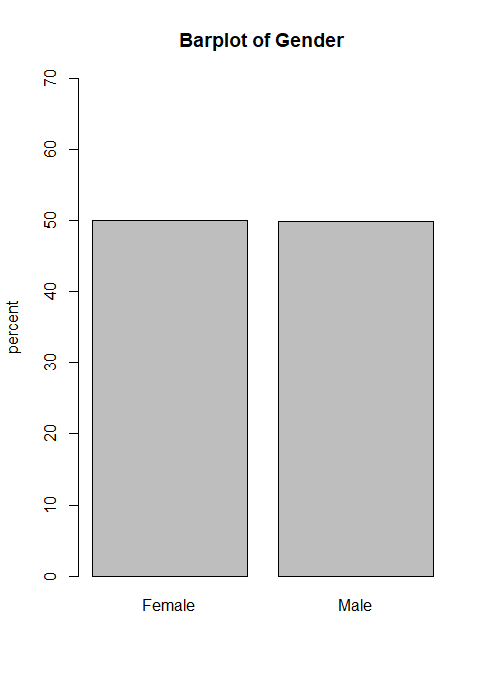
\includegraphics[width=0.5\linewidth]{screenshot006}
	\caption{Gender statistics barplot}
	\label{fig:genderbar}
\end{figure}
Figure \ref{fig:genderbar} shows a barplot of the gender. It shows that the males have a percentage of 49.9\%; a total of 499 and the females have a percentage of 50.1\%; a total of 501.
\section{The estimates of the fitted GLM models}
The parameters of the fitted  GLM model are estimated using the maximum likelihood estimation method. The fitting was done and summaries where total sales is the response variable.
A generalized linear model with Gamma distribution was fitted to the data and summary of estimates was obtained. 
\begin{table}[H]
\centering
\caption{Parameter estimates of the fitted Gamma model}	
	\begin{tabular}{ccccc}
		\hline
		Variable   & Parameter & se(parameter) & p-value & exp(parameter) \\ \hline
		Intercept  & 3.0425 & 0.0559     & 0.0000  & 20.9573        \\
		Unit price & 0.0209 & 0.0559     & 0.0000  & 1.0211         \\
		Quantity   & 0.2220 & 0.0070     & 0.0000  & 1.2485         \\
		Tax        & 0.0003 & 0.0023     & 0.8800  & 1.0003         \\
		Rating     & 0.0039 & 0.0051     & 0.4400  & 1.0039         \\
		Gender     & 0.0064 & 0.0175     & 0.7160  & 1.0064         \\ \hline
	\end{tabular}
\label{table:gamma}
\end{table}
 Table \ref{table:gamma} shows the estimated parameters of the total sales using GLM with Gamma model. The coefficient estimate in the output indicates the average change in the log odd of the response variable with a unit increase in each predictor variable for example, a unit increase in the predictor variable unit price is associated with an average change of 0.0208 in the log odds of the response variable. This means higher values of the unit price are associated with a higher likelihood of the response variable. The standard error  gives an idea of the  variability associated with coefficient estimate. This essentially tells us how well each predictor variable is able to predict the value of the response variable in the model. The variables unit price, quantity and tax are significant at 5\% level. The coefficients for unit price, quantity, rating, gender and tax estimates are positive indicating positive correlation with the response variable.
  
\begin{table}[H]
	\centering
	\caption{Parameter estimates of the fitted Inverse Gaussian model}
	\begin{tabular}{ccccc}
		\hline
		Variable   & Parameter  & se(parameter) & p-value & exp(parameter) \\ \hline
		Intercept  & 0.0215 & 0.0005     & 0.0000  & 1.0218         \\
		Unit price & -0.0002 & 0.0000     & 0.0000  & 0.9998         \\
		Quantity   & -0.0019 & 0.0001     & 0.0000  & 0.9981         \\
		Tax        & 0.0003 & 0.0000     & 0.0000  & 1.0003         \\
		Rating     & -0.0000 & 0.0000     & 0.4660  & 1.0000         \\
		Gender     & -0.0000 & 0.0001     & 0.7610  & 1.0000         \\ \hline
	\end{tabular}
\label{table:inverse}
\end{table}
Table \ref{table:inverse} shows the estimated parameters of the total sales using a GLM with Inverse Gaussian distribution. The p-value is used in checking the significant variables. The variables; unit price, quantity and tax are significant at 5\% level of significance. The significant variables shows there is correlation  with the response variable. The coefficients for unit price, quantity, rating and gender are negative implying negative correlation with the response variable while the coefficient for tax estimate is positive indicating positive correlation with the response variable. The standard error provides the absolute measure of the typical distance that the data points fall from the regression line. 

\begin{table}[H]
	\centering
	\caption{Parameter estimates of the fitted Gaussian model}
	\begin{tabular}{ccccc}
		\hline
		Variable   & Parameter & se(parameter) & p-value & exp(parameter) \\ \hline
		Intercept  & 0.0113    & 0.0004        & 0.0000  & 1.0113         \\
		Unit price & -0.0001   & 0.0000        & 0.0000  & 0.9999         \\
		Quantity   & -0.0008   & 0.0001        & 0.0000  & 0.9992         \\
		Tax        & 0.0001    & 0.0000        & 0.0000  & 1.0000         \\
		Rating     & 0.0000    & 0.0000        & 0.8320  & 1.0000         \\
		Gender     & 0.0000    & 0.0001        & 0.8960  & 1.0000         \\ \hline
	\end{tabular}
\label{table:Gaussian}
\end{table}
Table \ref{table:Gaussian} shows the estimated parameters of the total sales using GLM with Gaussian distribution. The coefficient estimate in the output indicates the average change in the response variable with a unit increase in each predictor variable for example, a unit increase in the predictor variable unit price is associated with an average change of -0.0001 in the response variable. This means that the higher values of the unit price are associated with lower values of the response.  The variables unit price, quantity and tax are significant at 5\% significance level. The coefficients for unit price and quantity are negative implying negative correlation with the response variable while the coefficient for tax estimate is positive indicating positive correlation with the response variable. The standard error  gives an idea of the  variability associated with coefficient estimate. For example the variability associated with unit price is 0.004.
\section{Model selection}
The AIC is a metric used to compare the fit of different regression models. The lower the value the better the regression model is able to fit the data. 
\begin{table}[H]
	\centering
	\caption{AIC values for selecting the model}
	\begin{tabular}{@{}cccc@{}}
		\toprule
		& Gamma & Inverse Gaussian & Gaussian \\ \midrule
		AIC & 8846  & 10183            & 9489     \\ \bottomrule
	\end{tabular}
\label{table:selection values}
\end{table}
Table \ref{table:selection values} shows the Akaike Information Criterion values for the three generalized linear models that is Gamma, Inverse Gaussian and Gaussian models. It can be seen that the model with inverse Gaussian has the highest value and the model with Gamma has the least AIC. This further implies that the Gamma model is considered to be a better fit for the data.
\section{Adequacy of the model}
To assess the adequacy of the fitted model, a Chi-square goodness of fit test at 5\% significance level was used. The model has a chi-square statistic 149019 and 799 degrees of freedom. The chi-square distribution returns a p-value of zero. Consequently the null hypothesis, in equation (\ref{eqn:chihypo}) is rejected at 5\% level of significance that the deviation between the observed and the expected is not significantly large and thus the model is a good fit to the data. 

\section{Prediction using the fitted model}
A GLM gamma model was chosen to forecast the sales. The gamma model took the equation of the form;
\begin{equation}
\centering
\label{eqn:forecasteqn}
	\hat{P}(Y|X) = \frac{exp((3.0420 + 0.0210 X_{1} + 0.2220 X_{2} + 0.0003 X_{3} + 0.0039 X_{4} + 0.0064 X_{5}))}{1+ exp(-(3.0420 + 0.0210 X_{1} + 0.2220 X_{2} + 0.0003 X_{3} + 0.0039 X_{4} + 0.0064 X_{5}))}
\end{equation}
where $g$ is the associated link function.
The Gamma GLM model was used to predict the sales and a sample of the predictions are given.
\begin{table}[H]
	\centering
	\caption{Actual and Predicted sales values}
	\begin{tabular}{lll}
		\hline
		No. & Actual  & Predicted \\ \hline
		801 & 144.963 & 133.514   \\
		802 & 253.680 & 238.089   \\
		803 & 495.317 & 421.726   \\
		804 & 462.672 & 446.291   \\
		805 & 714.326 & 781.299   \\
		806 & 325.374 & 262.224   \\
		807 & 195.678 & 236.977   \\
		808 & 210.966 & 151.038   \\ \hline
	\end{tabular}
\label{table:values}
\end{table}
Table \ref{table:values} shows the first eight values of the predicted and actual sales using GLM with Gamma model. The values show that the model generated values that reflect the actual values; implying that the forecasts were accurate. 
\begin{figure}[H]
	\centering
	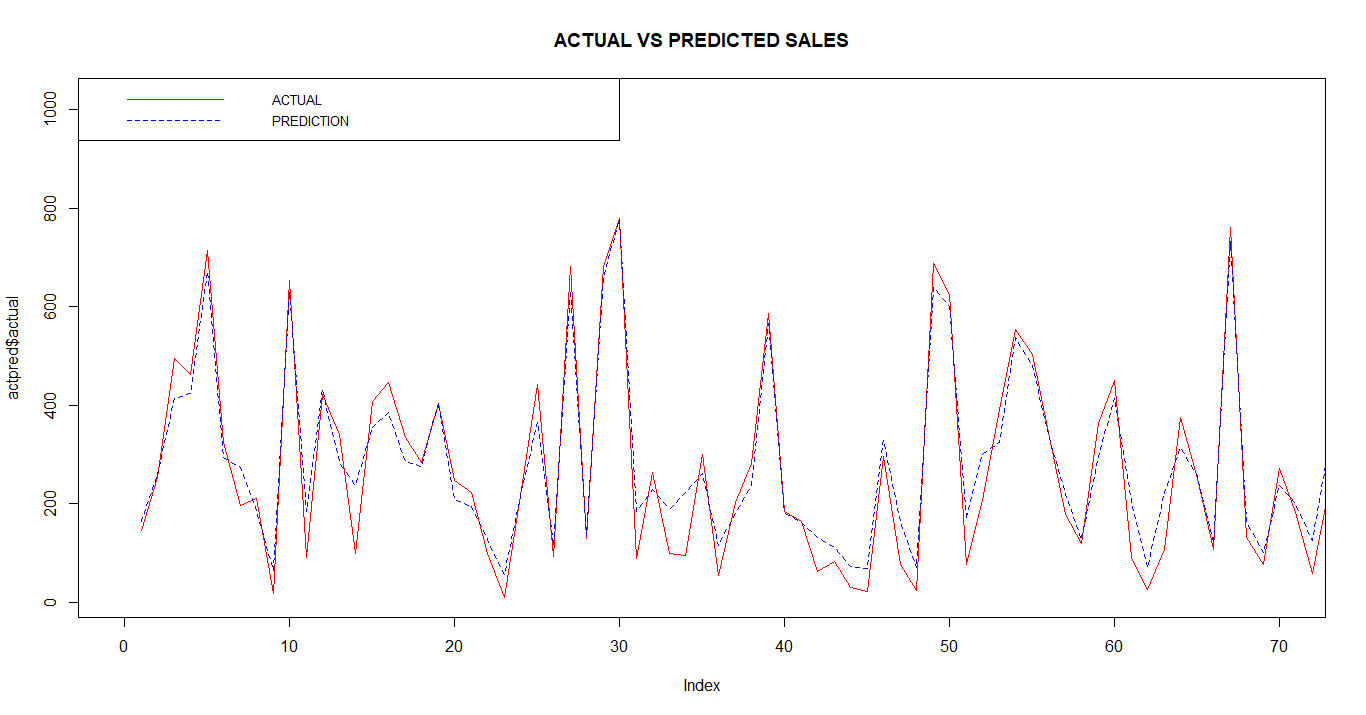
\includegraphics[width=0.9\linewidth]{screenshot005}
	\caption{Plot of Actual and predicted sales}
	\label{fig:plot accuracy}
\end{figure}

Figure \ref{fig:plot accuracy} shows the plot of the actual and forecasted sales. The plot shows that the sales forecast are not far from the actual observed sales. This shows that the GLM Gamma model fitted was a good choice for the sales data.
\section{The accuracy of the sales forecast}
 The accuracy of the sales forecast was checked using the mean square error formula in equation (\ref{eqn:MSE}).
 Mean square error measures the average of squares of errors. A large MSE indicates wide dispersion from the actual values while lower values indicates closeness to the actual values which further implies the prediction model is accurate. An MSE value of 0.0603 was obtained  which shows that the forecast were accurate.




\chapter{Summary and Conclusion} 
\label{Chapter5} 
\lhead{Chapter 5. \emph{Conclusion}} 
\setstretch{1.5} 
%----------------------------------------------------------------------------------------
\section{Introduction}
%This chapter covers the summary of the findings, conclusions drawn, recommendation and areas of further research. conclusions drawn are based on data analysis, discussions and results from the previous chapter.
This chapter gives the summary and conclusions made according to the obtained results of the sales forecast and also the recommendations of the study. Section 5.2 gives the summary of the results. Section 5.3 gives the conclusions drawn from the findings of this study. Section 5.4 outlines the recommendations suggested for further research.

\section{Summary}
The generalized linear models offers certain advantages over ordinary linear model: the separate specification for distribution and link function offers flexibility for achieving linearity, the link functions and its inverse functions allows for interpretation in both the transformed scale and original scale, it allows for specifications of distributions that explicitly model non normality when strict statistical assumptions are met and finally, allows for variety of research designs with any number of  potential predictors.
%In this study, sales of a supermarket have been fitted to generalized linear models with Gaussian, Gamma and inverse Gaussian each with log and inverse link functions respectively and the best model out of the three was selected based on least value of AIC. The Gamma model had the least AIC hence was chosen. Although a Gamma distribution fitted the data set well, there were a few product classes of which the model did not fit the distribution perfectly.\\
%Based on 5\% significance level and p value sales modeled using GLM Gamma passed the goodness of fit test using Chi-square and Wald tests. The adequate model was then  used to predict sales and sample of sales predictions have been given on table \ref{table:values}. In checking the accuracy of the predicted sales mean squared error was used and a value of 0.06 was obtained signifying good prediction capacity of the model.\\
%From the above findings it was noted that sales vary similarly with tax and varies inversely with unit price, quantity rating and gender. That is, an increase in tax will result in sales increase and conversely a decrease in unit price, quantity rating and gender increases the sales.\\

This study focused on fitting generalized linear models to the supermarket sales using the Gaussian, Gamma and Inverse Gaussian distributions;the Gaussian and Gamma both having the log link function and the Inverse Gaussian having the inverse link function. After the models were fitted, a suitable had to  be chosen. The Akaike Information Criterion was used in selecting a suitable model from the three model fits. The Gamma model proved to be the most suitable model since it had the least AIC.
The Gamma model fit coefficients were all positive indicating positive correlation to the response variable; sales. So as to use the model in forecasting, the model's adequacy had to be assessed.

A chi-square goodness of fit test was carried out at a 5\% level of significance to assess the Gamma model's adequacy. The chi-square test proved that the Gamma model was adequate to carry out the forecast. The model produced forecasts which were then assessed using the Mean square Error. The MSE showed that there was minimal error in the forecast hence the forecast was accurate.
\section{Conclusion}
%Since the cost of goods sold and the gross margin were not significant they should be interacted or integrated with other factors so as to uncover their impact on overall sales. These findings are a representative of parts of supermarkets and does not represent the general trend. However, the findings are beneficial to supermarkets since they are aimed at better risk or loss quantification thus better adjustment of the factors. In conclusion generalized linear model proved to be reliable  model in sales forecasting as it gave predicted sales values which are a reflection of the observed values. 
This study aimed at forecasting supermarket sales. These sales forecasts play an important role in helping the supermarkets to run and manage their day to day activities. Apart from supermarkets, the study can also be applied to other commercial institutions that deal with sales. From the findings a generalized linear model proved to be reliable in sales forecasting since it was easy to use, handled the data easily and it gave forecasted sales values which were a reflection of the actual sales values.  
\section{Recommendations for Further Research}
This study was based on supermarkets sales. A similar study is recommended for other commercial firms. Also, other exponential distributions instead of Gamma, Gaussian and Inverse Gaussian can be applied together with other predictor variables to evaluate their impact on total sales. One difficulty that reoccurred on several occasions during the pre-phase of the study was to handle the flaws of the structure of the initial data thus it recommends that constructing a better way of sorting and cleaning the initial data not only be time consuming actions be reduced but also the building of the model will benefit. Since shifts of customer interests is disregarded in this study and considering the rapid movements in the sector, for further research this study recommends adding more flexibility regarding behavior changing factors such as existing and future trends, campaigns and marketing when modeling.


\label{References}
\lhead{\emph{References}} 
\References
\printbibliography[title={References}]
Hothorn, T., Hornik, K., Zeileis, A. 2006. Unbiased Recursive Partitioning: A Conditional Inference
Framework. Journal of Computational and Graphical Statistics, 15(3), 651-674.\\
P. Jong, G. Z. Heller, “Generalized Linear Models for Insurance 
Data,” International Series on Actuarial Science, Cambridge 
University Press, 2008. \\
Razzaghi, M. 2013. The Probit Link Function in
Generalized Linear Models for Data Mining Applications. Journal of Modern Applied Statistical Methods, 12(19), 164-169.\\
Wamwea, Charity Mkajuma, Benjamin Kyalo Muema, Joseph Kyalo Mung’atu, et al. (2019). “Modelling a pay-as-you-drive insurance pricing structure using a generalized linear model: Case study
of a company in Kiambu”. In: American Journal of Theoretical and Applied Statistics 4.6, pp. 527–
533.\\
Friedman, J., Hastie, T., Tibshirani, R. 2010. Regularization Paths for Generalized Linear Models via Coordinate Descent. Journal of Statistical Software, Articles, 33(1), 1-22.\\

\appendix
\titleformat{\chapter}[hang]
{\filleft\huge} {} {0ex} {\bfseries}%\MakeUppercase
\titlespacing*{\chapter}
{0pt} {-50pt} {5pt}
\chapter{Appendix} 
\label{Appendix}
\lhead{Appendix: \emph{Proposed Budget}}
\section{Proposed Budget}


\newpage
\lhead{Appendix: \emph{Project Work Plan}}
\section{Project Work Plan}
	\begin{ganttchart}[
	today=15,
	today rule/.style= {blue, thick},
	x unit=0.39cm,
	y unit title=01cm,
	y unit chart=0.8cm,
	title label font=\normalsize,
	bar label font=\normalsize,
	group label font=\normalsize\bfseries,
	milestone label font=\normalsize\itshape,
	vgrid={*{3}{gray!60, dashed}, *1{black}},  hgrid]  {1}{32}
	\gantttitle{2020}{32} \\		
	\gantttitle{May}{4}
	\gantttitle{Jun}{4}
	\gantttitle{Jul}{4}
	\gantttitle{Aug}{4}
	\gantttitle{Sep}{4}				
	\gantttitle{Oct}{4}
	\gantttitle{Nov}{4}
	\gantttitle{Dec}{4} \\
	
	\ganttbar[bar/.append style={fill=blue!10}]{Concept Writing}{1}{4} \\
	\ganttmilestone{Concept Presentation}{5}\\
	
	\ganttbar[bar/.append style={fill=blue!10}]{Introduction}{4}{8} \\
	\ganttbar[bar/.append style={fill=blue!10}]{Literature Review}{8}{12} \\
	\ganttbar[bar/.append style={fill=blue!10}]{Methodology}{12}{18} \\
	
	\ganttmilestone{Proposal Presentation}{19}\\
	
	\ganttbar[bar/.append style={fill=blue!40}]{Writing R Codes}{19}{20} \\
	\ganttbar[bar/.append style={fill=blue!40}]{Testing R codes}{21}{22}\\
	\ganttbar[bar/.append style={fill=blue!40}]{Results}{21}{25}\\
	\ganttbar[bar/.append style={fill=blue!40}]{Discussion}{25}{28} \\			
	\ganttbar[bar/.append style={fill=blue!40}]{Conclusion}{29}{29} \\
	
	\ganttmilestone{Project Presentation}{30}
	
	\ganttlink{elem0}{elem1}
	\ganttlink{elem1}{elem2}
	\ganttlink{elem2}{elem3}
	\ganttlink{elem3}{elem4}
	\ganttlink{elem4}{elem5}
	\ganttlink{elem5}{elem6}
	\ganttlink{elem6}{elem7}
	\ganttlink{elem7}{elem8}
	\ganttlink{elem8}{elem9}
	\ganttlink{elem9}{elem10}
	\ganttlink{elem10}{elem11}
\end{ganttchart}

%\newpage
%\lhead{Appendix. \emph{R Program Codes}}
%\section{R Program Codes}

\backmatter
\end{document} 

